\section{Ray-marching - Maximum number of iterations vs. distance threshold
	condition}\label{ray-marching---maximum-number-of-iterations-vs.-distance-threshold-condition}

The \emph{ray marching distance threshold} is the condition where the photon
marching along the ray comes within a specified distance from the fractal
surface and the ray-marching stops. This controls the size of the detail in the
image, and is normally set to vary such that greater detail is obtained for the
surface closest to the camera, (in the further regions of the fractal the
distance threshold will be larger such that only bigger details are visible).
Enabling \emph{Constant Detail Size} on the \emph{Rendering Engine} tab will
make the distance threshold uniform.

There are two modes of stopping the ray-marching of each image pixel.

1st case: Stop ray-marching at distance threshold (\emph{Stop at maximum
	iteration} is disabled).

2nd case: Stop ray-marching at point when a maximum number of iterations is
reached (\emph{Stop at maximum iteration} is enabled).

First important note: \emph{Stop at maximum iteration} doesn't control the
fractal iteration loop. It controls only ray-marching. The iteration loop always
runs to achieve Bailout, (then if bailout is not reached the iteration stops at
Maxiter).

Example for 1st case - stop ray-marching at distance threshold: \nopagebreak

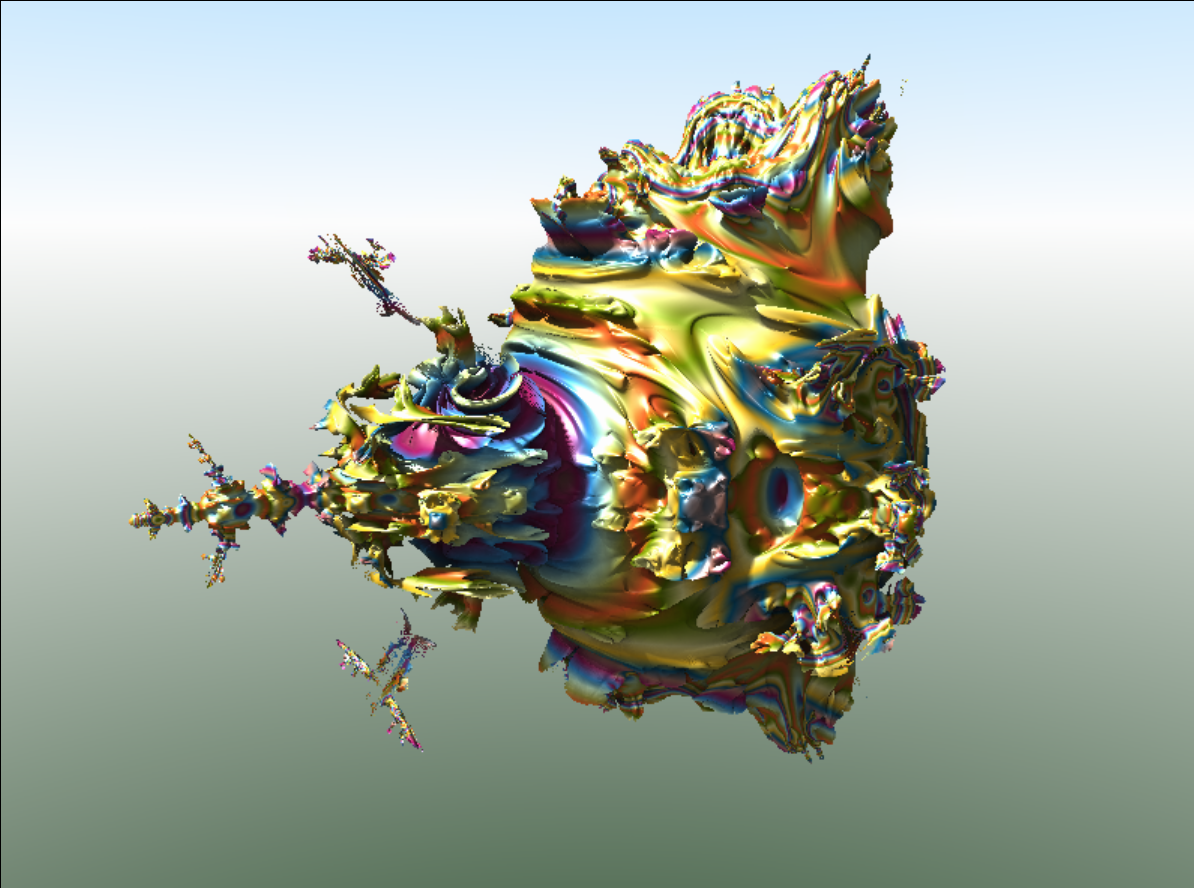
\includegraphics[width=0.5\linewidth]{img/manual/media/stop_raymarching_at_disttrhersh}

Ray-marching stops at distance threshold. In most cases the fractal iteration
loop stops on bailout condition, (because away from surface it is not possible
to reach Maxiter). It makes rendering of fractals much faster.

Example for 2nd case: Stop ray-marching at Maxiter \nopagebreak

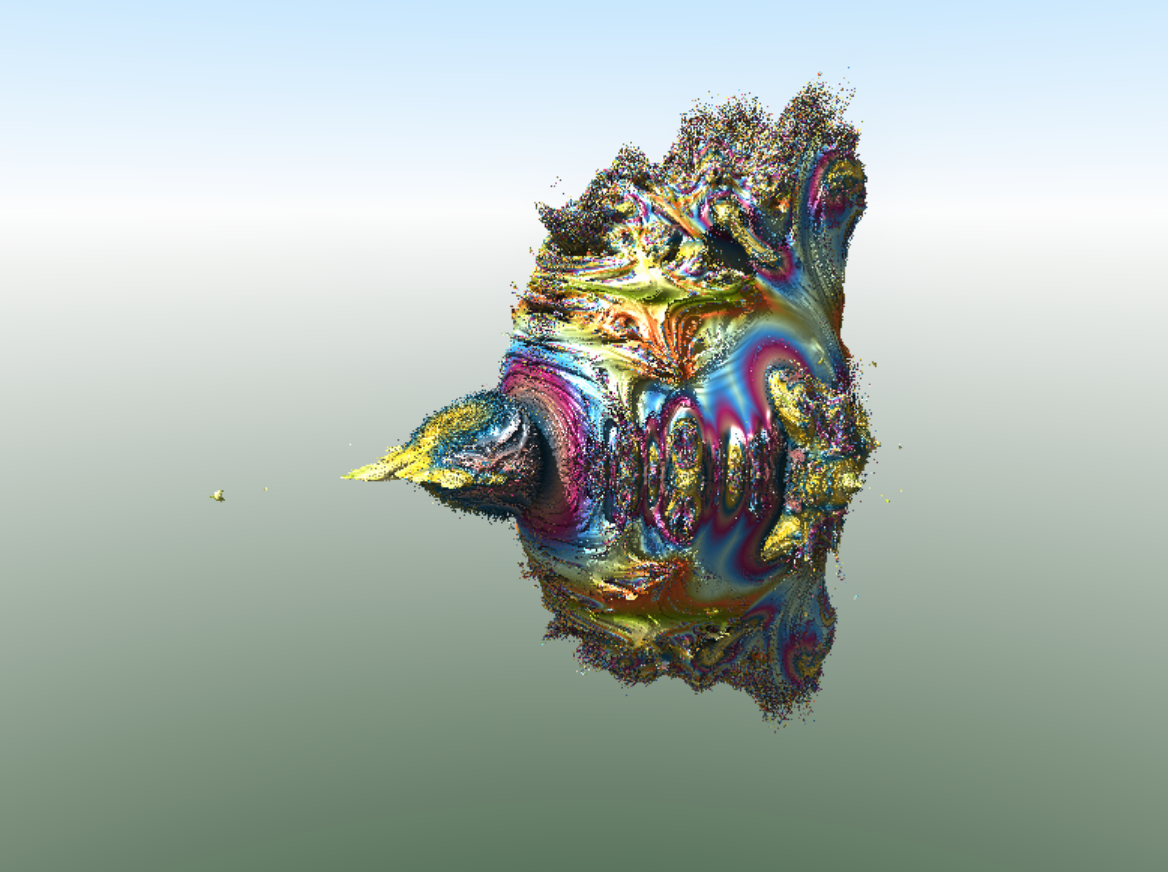
\includegraphics[width=0.5\linewidth]{img/manual/media/stop_raymarching_at_maxiter}

Ray-marching stops at the photon step when the maximum number of iterations is
reached (ray-marching distance threshold is ignored). In many cases iteration
loop stops on bailout condition (away from fractal surface), but on the fractal
surface the maximum number of iterations is calculated (when bailout is not
reached).

Example for 1st case: Stop ray-marching at bailout with low Maxiter \nopagebreak

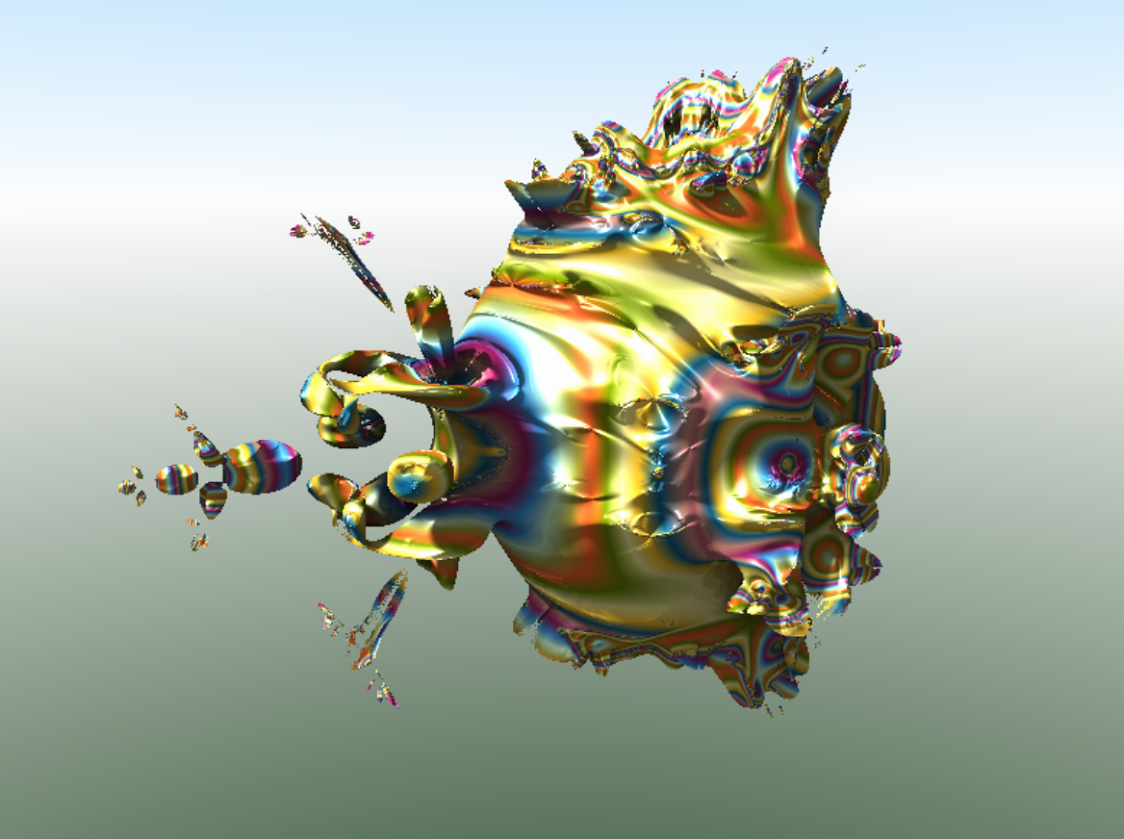
\includegraphics[width=0.5\linewidth]{img/manual/media/stop_raymarching_at_disttrhersh_iter4}

When maximum number of iterations is set to 4. Even if Maxiter is reached the
ray-marching is continued until the ray marching distance threshold is reached.


Example for 2nd case: Stop ray-marching at maxiter with low maxiter \nopagebreak

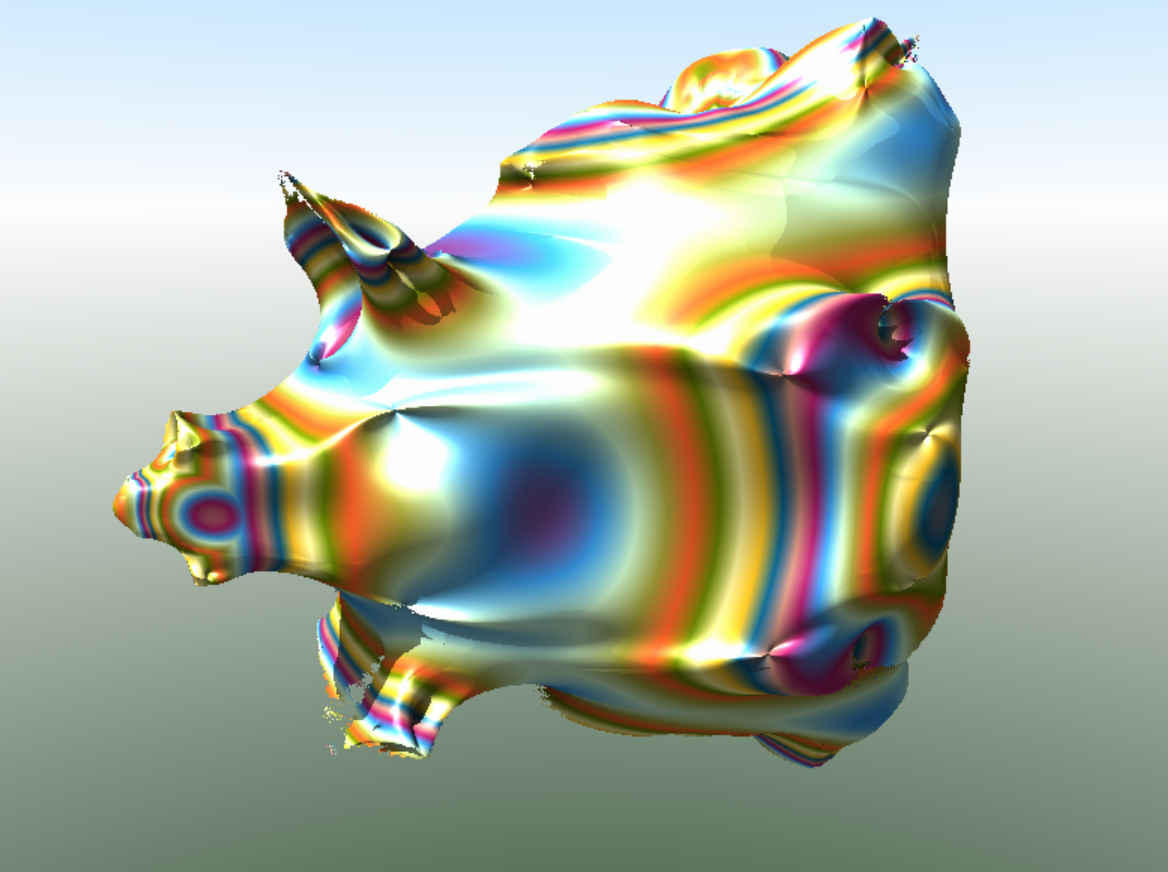
\includegraphics[width=0.5\linewidth]{img/manual/media/stop_raymarching_at_maxiter_iter4}

When maximum number of iterations is reached, then ray-marching is stopped even
if distance threshold is not reached.


